\documentclass[a4paper,oneside,12pt]{book}
\usepackage{BUPTthesisbachelor}
\usepackage{setspace}
\usepackage{adjustbox}



%\lstdefinestyle{sharpc}{language=[Sharp]C, frame=lrtb, rulecolor=\color{blue!80!black}}


%%%%%%%%%%%%%%%%%%%%%%%%% Begin Documents %%%%%%%%%%%%%%%%%%%%%%%%%%
\begin{document}

% 封面

\includepdf[pages=-]{docs/cover.pdf}  
\newpage

% 任务书
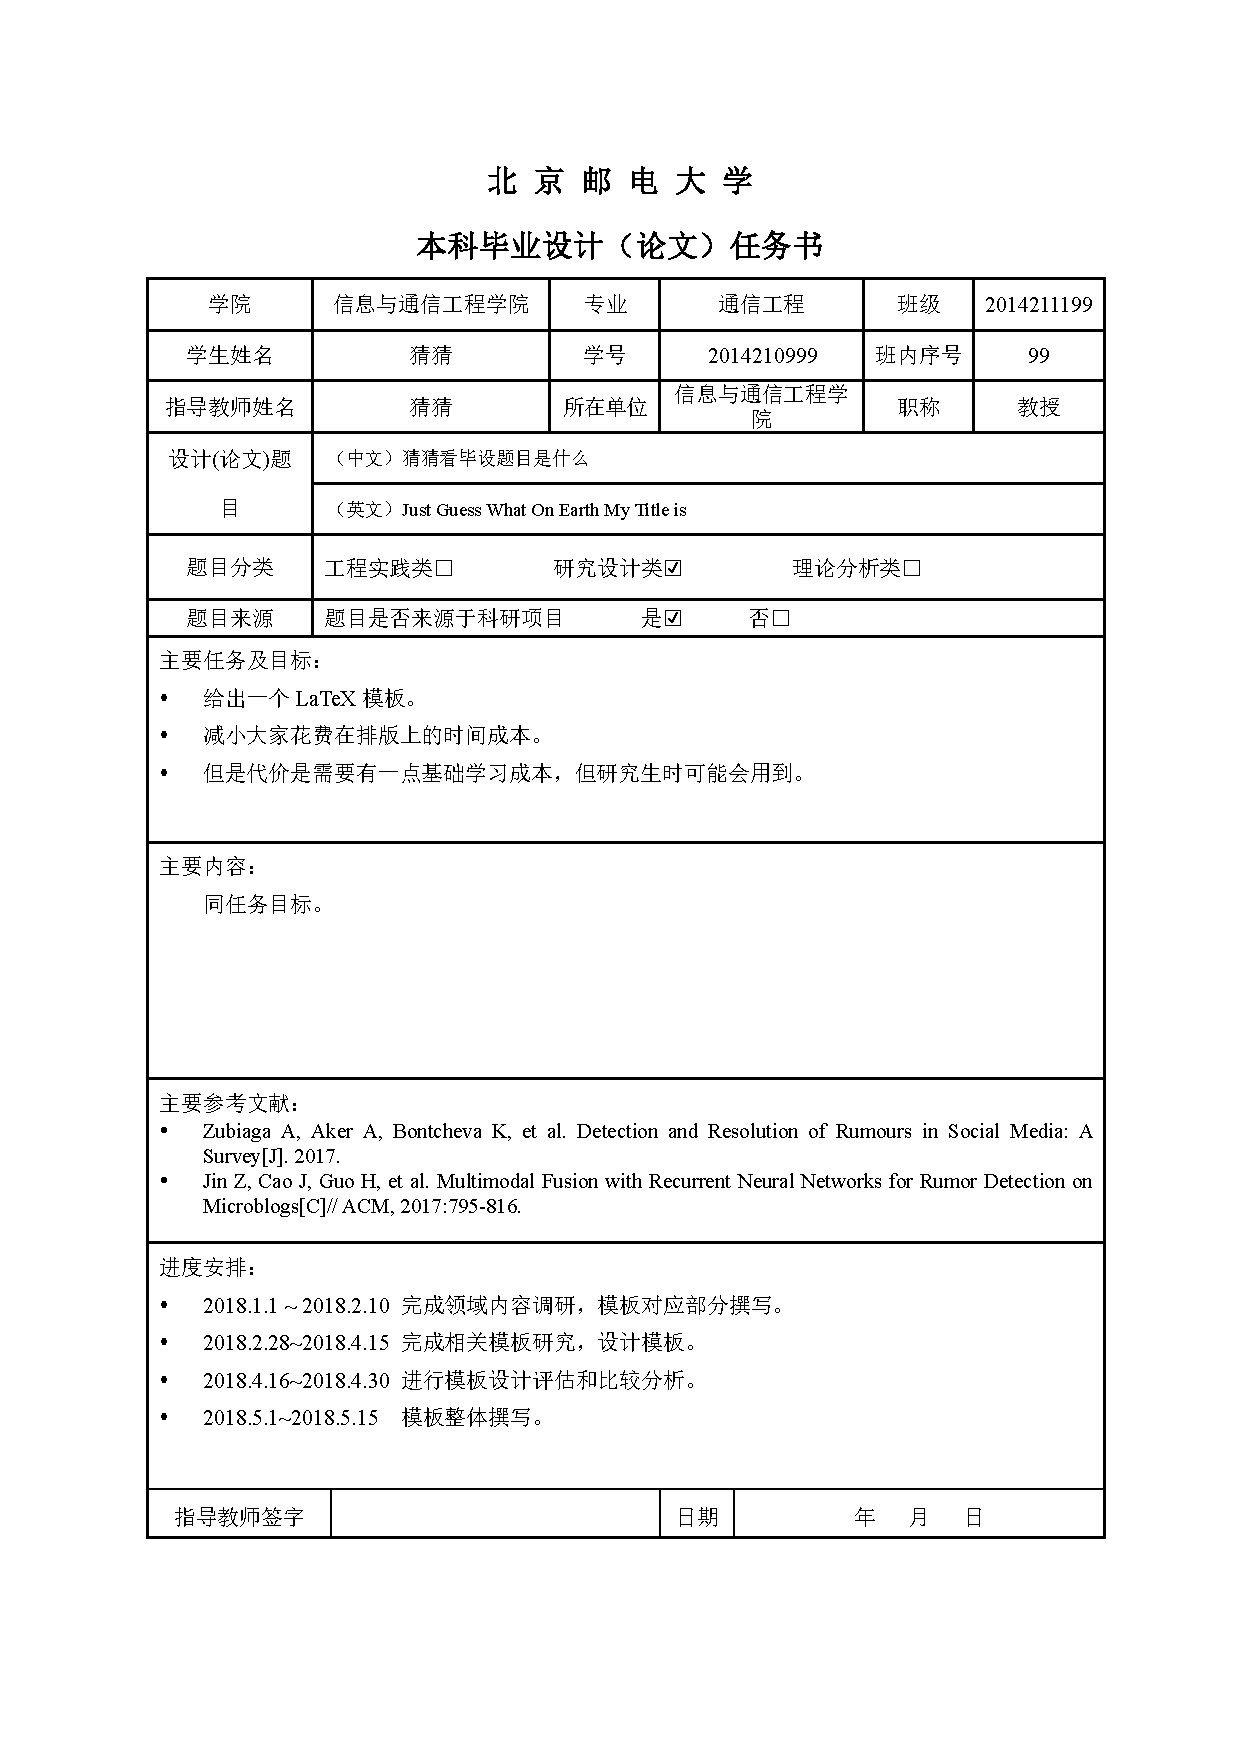
\includepdf[pages=-]{docs/task.pdf}  
\newpage

% 成绩评定表
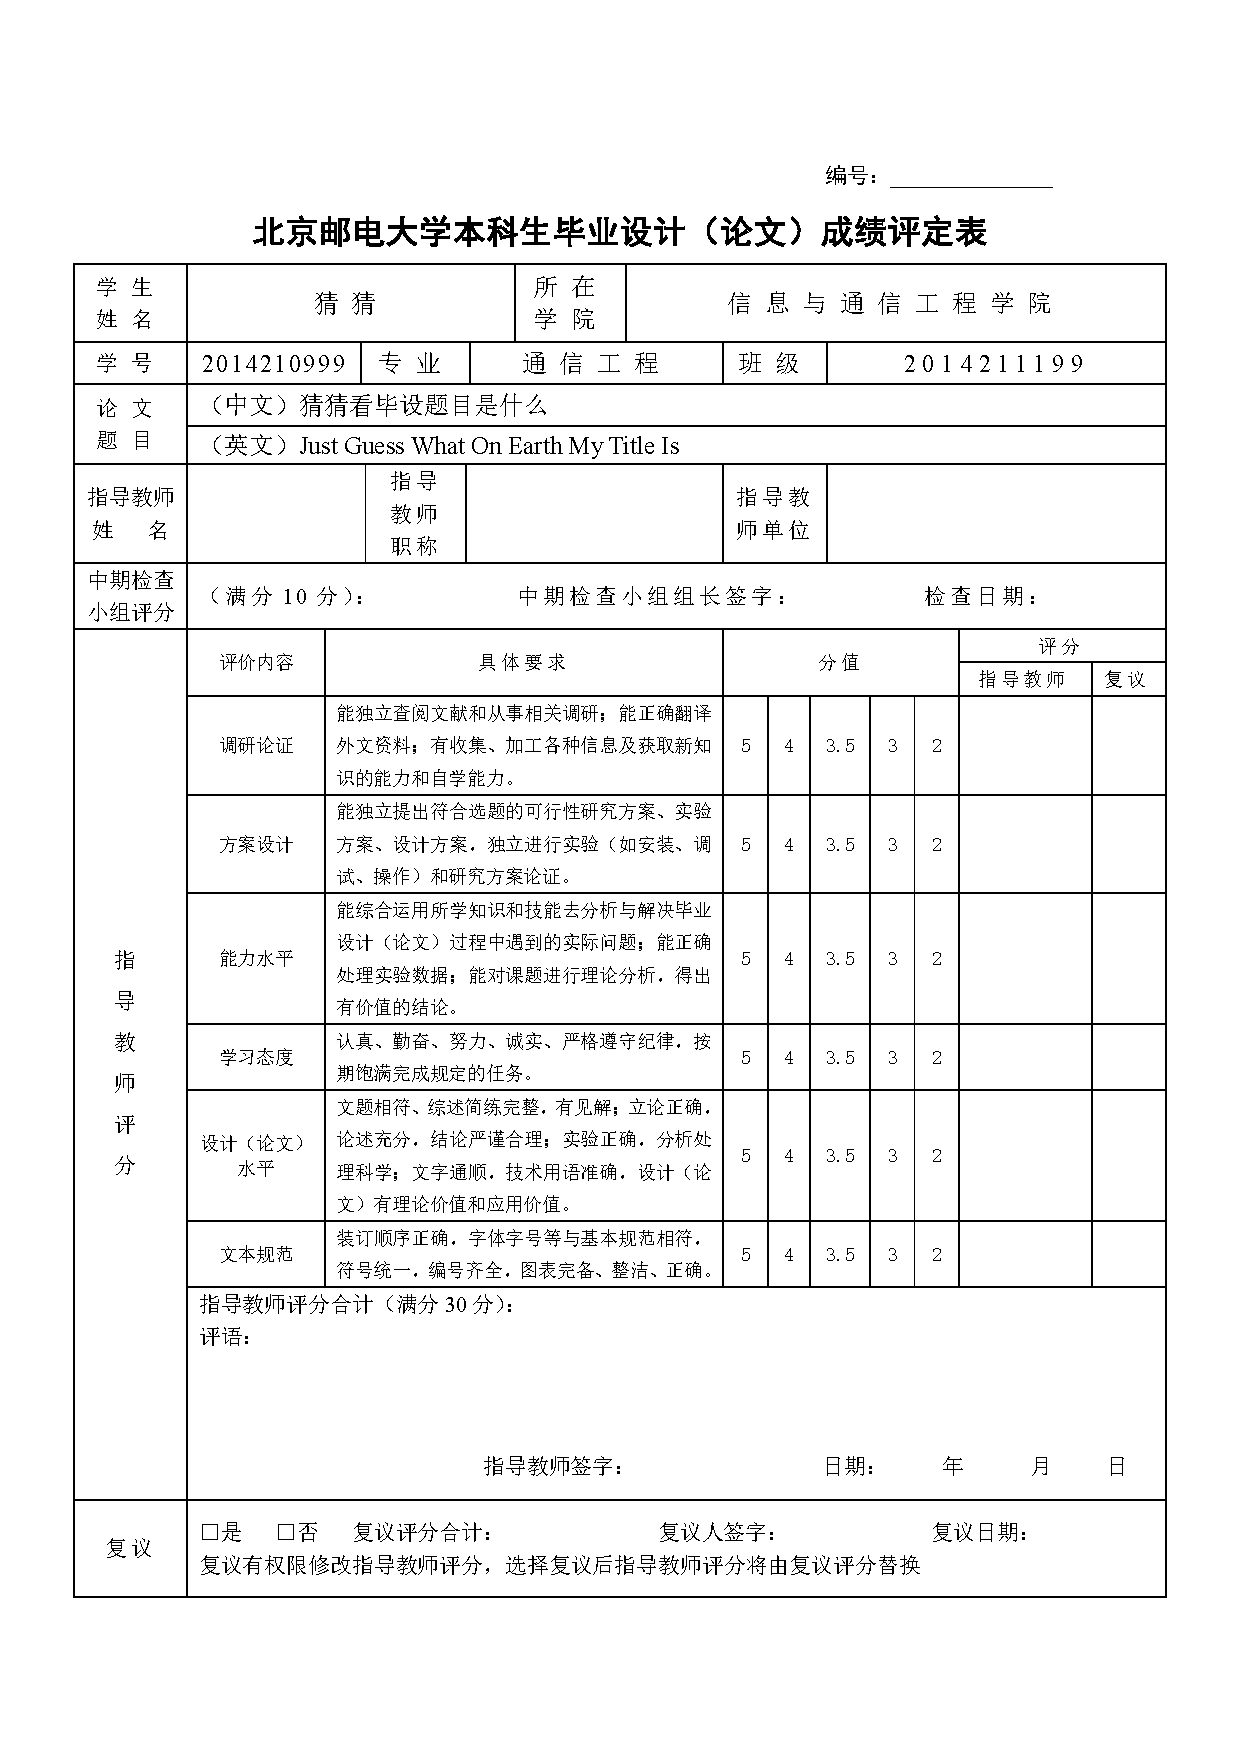
\includepdf[pages=-]{docs/scoreTable.pdf}  
\newpage

% 诚信声明

\includepdf[pages=-]{docs/statement.pdf} 
\newpage

%%%%%%%%%%%%%%%%%%%%%%%%%%%%%%%%%%%%%%%%%%%%%%%%%%%%%%%%%%%%%%%%%%%%
%                                                                  %
%   Copyright (c) 2010 - 2011 Caspar Zhang <casparant@gmail.com>   %
%                                                                  %
%   This copyrighted material is made available to anyone wishing  %
%   to use, modify, copy, or redistribute it subject to the terms  %
%   and conditions of the GNU General Public License version 2.    %
%                                                                  %
%   This program is distributed in the hope that it will be        %
%   useful, but WITHOUT ANY WARRANTY; without even the implied     %
%   warranty of MERCHANTABILITY or FITNESS FOR A PARTICULAR        %
%   PURPOSE. See the GNU General Public License for more details.  %
%                                                                  %
%   You should have received a copy of the GNU General Public      %
%   License along with this program; if not, write to the Free     %
%   Software Foundation, Inc., 51 Franklin Street, Fifth Floor,    %
%   Boston, MA 02110-1301, USA.                                    %
%                                                                  %
%%%%%%%%%%%%%%%%%%%%%%%%%%%%%%%%%%%%%%%%%%%%%%%%%%%%%%%%%%%%%%%%%%%%

% 你只需要修改下面几行就可以完成大部分内容的填写,
% 这要求你具有一定的LaTeX基础,但是如果你足够聪明,
% 不具有LaTeX基础也可以完成。

% 论文中文题目
\def\thesistitle{社猜猜看这个毕设题目是什么}

% 论文英文题目
\def\thesistitleen{Have a try to guess what the title is}

% Thank Words
\def\thankwords{

此处请写致谢的内容。

它可以有多段。
}
    % Main items 
%%%%%%%%%%%%%%%%%%%%%%%%%%%%%%%%%%%%%%%%%%%%%%%%%%%%%%%%%%%%%%%%%%%%
%                                                                  %
%   Copyright (c) 2010 - 2011 Caspar Zhang <casparant@gmail.com>   %
%                                                                  %
%   This copyrighted material is made available to anyone wishing  %
%   to use, modify, copy, or redistribute it subject to the terms  %
%   and conditions of the GNU General Public License version 2.    %
%                                                                  %
%   This program is distributed in the hope that it will be        %
%   useful, but WITHOUT ANY WARRANTY; without even the implied     %
%   warranty of MERCHANTABILITY or FITNESS FOR A PARTICULAR        %
%   PURPOSE. See the GNU General Public License for more details.  %
%                                                                  %
%   You should have received a copy of the GNU General Public      %
%   License along with this program; if not, write to the Free     %
%   Software Foundation, Inc., 51 Franklin Street, Fifth Floor,    %
%   Boston, MA 02110-1301, USA.                                    %
%                                                                  %
%%%%%%%%%%%%%%%%%%%%%%%%%%%%%%%%%%%%%%%%%%%%%%%%%%%%%%%%%%%%%%%%%%%%

% 你只需要修改下面内容就可以完成中英文摘要,
% 这要求你具有一定的LaTeX基础,但是还是那句话,
% 如果你足够聪明,不具有LaTeX基础也可以完成。

% 中文摘要
\def\abstractcn{
%从这里开始写你的摘要,分段需要空一行。
这是中文摘要的部分。

它可以拥有多段。
%摘要结束
}

% 中文关键字 
% TODO: 改成可变长度的
\def\abscnkeyone{北京邮电大学}
\def\abscnkeytwo{本科生}
\def\abscnkeythree{毕业设计}
\def\abscnkeyfour{模板}
\def\abscnkeyfive{示例}

% ABSTRACT
\def\abstracten{
%Your abstract here, to make a new paragraph, give an extra blank line please.
This is ABSTRACT.

You can write more than one paragraph here.
%Abstract done
}

% Key Words 
% TODO: 改成可变长度的
\def\absenkeyone{BUPT}
\def\absenkeytwo{undergraduate}
\def\absenkeythree{thesis}
\def\absenkeyfour{template}
\def\absenkeyfive{example}


  % Abstract
\frontmatter\tableofcontents % Content

% 正文
\newpage\mainmatter
\fancypagestyle{plain}{\pagestyle{fancy}} % Add head to new chapter
\pagestyle{fancy} % Head and foot
%\let\cleardoublepagebak=\cleardoublepage
%\let\cleardoublepage\relax % Make new chapter stay on old page

%%%%%%%%%%%%%%%%%%%%%%%%%%%%% Main Area %%%%%%%%%%%%%%%%%%%%%%%%%%%%
%% 简介
\chapter{绪论}
%\section{课题背景}

%社交媒体是一种供用户创建在线社群来分享信息、观点、个人信息和其它内容(如视频)的电子化交流平台,社交网络服务(social network service, SNS)和微博客(microblogging)都属于社交媒体的范畴\cite{webster_social_media},国外较为知名的有Facebook\footnote{http://www.facebook.com/}、Instagram\footnote{https://www.instagram.com/}、Twitter\footnote{http://www.twitter.com/}、LinkedIn\footnote{http://www.linkedin.com/}等,国内较为知名的有新浪微博\footnote{http://www.weibo.com/}。

说话人识别(Speaker Verification, SV)是指通过对说话人语音中的声学信息进行分析,自动识别说话人身份的一种技术。说话人识别在日常生活的各个领域都有着十分广泛的应用,有着至关重要的作用与广阔的市场。实现说话人识别系统,需要结合数字信号处理,模式识别等多学科的知识,是一个十分复杂的研究课题。截止目前,说话人识别相关技术的研究以及趋近成熟,在近些年也越来越多的投入商用。其中,GMM-UBM(Gaussian Mixture Model-Universal Background Model)系统\cite{reynolds2000speaker}和i-Vector系统\cite{dehak2011front}表现最为出色,成为了说话人识别领域中最为常用的两个系统。但是,虽然说话人识别的相关研究已经取得了很好的效果,当把这些研究成果应用于实际环境的时候,仍然有很多需要解决的问题。比如经研究表明,在复杂的噪声环境下说话人识别系统的准确率会大大下降\cite{yan2016improved}。因此,如何提升说话人识别系统在噪声环境下的说话人识别准确率便成了十分重要的研究课题。

说话人识别系统的结构主要分为三部分,特征提取,模型运算,及匹配判决。在近几十年的说话人识别研究过程中,有很多研究者对不同的部分进行改进,并提升说话人识别系统在噪声环境下的说话人识别准确率。在判决和模型部分,将无噪声语音信息和有噪声语音信息结合的多环境条件训练模型,可以有效的提高说话人系统在复杂噪声环境下的说话人识别准确率\cite{lei2013noise}。在前端特征提取中,很多语音增强模型被利用在说话人识别系统的特征提取过程中,以最大限度的降低噪音对于原本说话人语音的影响\cite{erkelens2007minimum}。

%\begin{definition}
%\end{definition}

以此同时,近些年深度神经网络(Deep neural networks, DNN)的热潮席卷整个计算机领域,在计算机视觉,自然语言处理等方向上,深度神经网络有着极其出色的作用,大大的推动了相关技术的发展及其商用\cite{lecun2015deep}。同时,在语音领域,深度神经网络也有着广泛的应用,应用深度神经网络的语音识别模型有着出色的效果\cite{hinton2012deep}。随着深度神经网络及类型的方法在语音领域的成功,也有很多研究者尝试在说话人识别领域应用这项技术。2014年首次有人提出了加入深度神经网络代替GMM的说话人识别模型\cite{lei2014novel},以提升说话人识别准确率。同年,谷歌的研究人员也推出了完全使用深度学习的d-vector说话人识别模型\cite{variani2014deep},并且在之后的几年中不断的更新着自己的模型,达到了不错的效果。但是截至目前,传统的GMM-UBM和i-vector模型仍然在说话人识别系统中占据主流地位,有着更好的效果。而且噪声等环境因素对于说话人模型的影响,要大于模型的选择,如何更好的提升噪声环境下的准确率才是当务之急。所以研究者们更多的着眼于用深度神经网络进行前端特征处理的工作,通过改进特征处理环节,尽可能减小噪声对于说话人识别模型的干扰\cite{xu2015regression}\cite{kolbk2017speech},而在后端模型的选择上,依然选择传统的隐变量模型。

随着深度学习的火热,更多衍生的深度神经网络模型被提出,其中,2014年Goodfellow等人提出的生成对抗网络(Generative Adversarial Nets,GAN)受到了广泛的关注\cite{goodfellow2014generative},因为其对抗训练的效果极其出色,GAN很快就被运用于图像生成处理等方向上。在语音处理领域,对抗网络也被用于搭建鲁棒语音识别模型\cite{shinohara2016adversarial}和语音生成\cite{mogren2016c}等研究中。


基于以上的背景,本课题的研究重点是神经网络特征在说话人认证系统中的鲁棒性,研究如何借助深度神经网络的方法,提取说话人鲁棒语音特征,使通过这些特征训练的说话人识别系统,在噪声环境下的说话人识别准确率提升。本文的主要安排如下。第一章绪论主要介绍课题的背景与研究的意义;第二章主要介绍课题中使用的基于深度神经网络的模型结构及其原理;第三章主要介绍实验准备,实施的具体内容;第四章主要是对实验结果进行介绍并分析;第五章将得出本文的结论。


%\section{相关研究的发展与最新进展}


%本文方法
\chapter{基于深度神经网络的鲁棒语音特征提取模型}

说话人识别系统主要的结构主要分为三部分,特征提取,模型运算,及匹配判决。特征提取部分被认为是整个系统的前端(front-end),提取的特征需要能包含说话人语音的个性信息,梅尔倒谱系数(MFCCs)\cite{davis1990comparison}是目前最为常用的特征参数,这种倒谱参数在上世纪八十年代被提出并用于语音识别,具有较好的鲁棒性,虽然有很多新特征不断的被提出,但是MFCCs目前很难被取代,本文也将会使用从语音数据中提取的MFCCs特征参数。 本文的研究也着重与前端部分,研究如何构造基于深度神经网络的鲁棒语音特征提取,并对他们的性能进行比较评价。

\section{瓶颈鲁棒语音特征}

MFCCs作为最广泛应用的特征参数,应用于说话人识别系统中有两个缺点。第一个缺点是MFCCs是在很短的语音段内被提取出来的,而部分说话人特征只有对相对更长的语音进行分析才能得到,因此使用MFCCs可能不能很好的表征部分说话人特征。第二个缺点是,MFCCs是为了语音识别而被设计出来的,虽然MFCCs也被证明可以用于说话人识别领域,但是它并不是最适合说话人识别系统的特征。因此,瓶颈特征被提了出来并应用于了说话人识别系统\cite{fu2014tandem}。将从说话人语音中提取出来的MFCCs特征,放入神经网络模型中训练,并在特定的隐藏层提取出来,便得到了瓶颈语音特征。提取的瓶颈特征能够更有效的表征长时间段语音的特征,并且通过神经网络训练的特征还能更加适应说话人识别任务。因此瓶颈特征可以很好的弥补上述MFCCs的缺点,更加适用于说话人识别系统,并在相关的研究中已经得到了证明\cite{liu2015deep}。

\section{深度神经网络鲁棒语音特征提取模型}

\section{对抗神经网络鲁棒语音特征提取模型}

\section{基准模型}

\subsection{STSA-MMSE}

\subsection{DNN based speech enhancement}

\subsection{SDN-BN}

\subsection{DAN-BN}

%实验,数据集,说话人识别系统
\chapter{实验}
\section{数据集}
\section{噪音}
\section{说话人识别系统}
\section{实验准备}


%结果与分析
\chapter{结果与分析}



损失函数变化曲线图
特征图谱
说话人识别等错率

 

\begin{table}
\renewcommand{\arraystretch}{1.0}
\caption{ EER ($\%$) of the ASV system using different front-ends on different noise types and SNRs (dB) }
\label{tab:clean}
%\begin{adjustbox}{max width=0.48\textwidth}
\begin{tabular}{| c | c | c | c| c|c| c| c|c|}
\hline
noise   &SNR  &No Enh. &MMSE &DNN-SE &SD-BN &SAN-BN & DAN-BN & MAN-BN\\
\hline
      & 00 &45.90 &30.95 &40.14 &27.89 & 27.02 &27.55 &\textbf{26.87}   \\ 
      & 05 &43.20 &21.17 &21.77 &18.80 &17.81 &18.37 & \textbf{17.69}   \\ 
      & 10 &34.61 &13.95 & \textbf{10.88} &11.26 &11.35 &12.61 &11.39   \\ 
White  & 15 &26.28 &10.20 &8.16 &7.51 &7.51 &7.17 & \textbf{6.83}   \\ 
      & 20 &16.91 &8.50 &6.80 &5.68 &5.29 & 5.44 &\textbf{5.10}   \\ 
      & clean &6.99 &5.80 &5.67 &4.08 &3.41 &3.66 & \textbf{3.29}   \\ 
\cline{2-9}     
      & mean &28.98 &15.10 &15.57 &12.54 &12.07 &12.47 & \textbf{11.86}   \\ 
 \hline 
      & 00 &19.05 &29.04 &16.67 & \textbf{13.60} &17.87 &15.99 &15.65   \\ 
      & 05 &14.63 &20.40 &10.39 &7.80 &9.86 &\textbf{8.16} & 8.35   \\ 
      & 10 &11.69 &12.59 &7.50 &5.10 &5.44 &4.76 & \textbf{4.07}   \\ 
Babble  & 15 &11.04 &7.82 &6.34 &4.25 &3.06 &3.74 & \textbf{2.94}   \\ 
      & 20 &9.18 &6.29 &5.78 &3.74 &3.40 &3.61 & \textbf{2.69}   \\ 
      & clean &6.99 &5.80 &5.67 &4.08 &3.41 &3.66 & \textbf{3.29}   \\ 
\cline{2-9}
      & mean &12.10 &13.66 &8.73 &6.43 &7.17 &6.65 & \textbf{6.16}   \\ 
 \hline 
      & 00 &20.72 &19.09 &19.94 &9.24 &9.81 &\textbf{9.18} & 10.54   \\ 
      & 05 &19.20 &12.37 &9.18 &6.00 &5.86 &\textbf{5.78} & 5.81   \\ 
      & 10 &14.74 &8.16 &6.12 &4.08 &4.44 &3.96 & \textbf{3.74}   \\ 
Cantine  & 15 &11.81 &6.80 &5.78 &3.86 &3.06 &3.40 & \textbf{3.03}   \\ 
      & 20 &8.50 &6.12 &5.44 &3.77 &3.40 &3.74 & \textbf{3.06}   \\ 
      & clean &6.99 &5.80 &5.67 &4.08 &3.41 &3.66 & \textbf{3.29}   \\ 
\cline{2-9}
	& mean &13.66 &9.72 &8.69 &5.17 &5.00 &4.95 & \textbf{4.91}   \\ 
 \hline 
      & 00 &29.40 &25.51 &21.77 & \textbf{11.94} &14.43 &13.50 &13.52   \\ 
      & 05 &20.07 &17.35 &10.59 & \textbf{6.46} &7.82 &6.80 &6.80   \\ 
      & 10 &15.00 &11.90 &7.48 & \textbf{3.17} &4.42 &4.78 &3.75   \\ 
Market  & 15 &11.96 &8.28 &6.22 &3.40 &3.62 &3.74 & \textbf{3.06}   \\ 
      & 20 &8.93 &7.35 &5.76 &3.74 &3.40 &3.40 & \textbf{2.80}   \\ 
      & clean &6.99 &5.80 &5.67 &4.08 &3.41 &3.66 & \textbf{3.29}   \\ 
\cline{2-9}    
    & mean &15.39 &12.70 &9.58 & \textbf{5.47} &6.18 &5.73 &5.53   \\ 
 \hline 
      & 00 &21.09 &17.69 &15.99 & \textbf{7.14} &9.86 &8.50 &8.09   \\ 
      & 05 &15.99 &12.58 &8.99 & 4.81 &6.46 &\textbf{4.76} &\textbf{4.76}   \\ 
      & 10 &13.61 &8.17 &6.12 & 3.75 &5.10 &\textbf{3.32} &3.68   \\ 
Airplane  & 15 &11.66 &6.53 &6.12 &3.67 &4.08 &3.40 & \textbf{3.06}   \\ 
      & 20 &9.18 &6.27 &5.58 &3.40 &3.63 &3.28 & \textbf{3.02}   \\ 
      & clean &6.99 &5.80 &5.67 &4.08 &3.41 &3.66 & \textbf{3.29}   \\ 
\cline{2-9}      
      & mean &13.09 &9.51 &8.08 &4.47 &5.42 &4.48 & \textbf{4.31}   \\ 
\hline
\end{tabular}
%\end{adjustbox}
\end{table}


%结论
\chapter{结论}


\iffalse
\section{图表及其引用}


此处引用了一张图。图\ref{autoencoder}表示的是一个由含有4个神经元的输入层、含有3个神经元的隐藏层和含有4个神经元的输出层组成的自编码器,$+1$代表偏置项。

\buptfigure{pictures/autoencoder}{自编码器结构}{autoencoder}





对中心化后的样本点集$\bm{X}=\{\bm{x}_1,\bm{x}_2,\ldots,\bm{x}_i,\ldots,\bm{x}_m\}$(有$\sum_{i=1}^{m}\bm{x}_i = 0$),考虑将其最大可分地投影到新坐标系\ $\bm{W}= \{\bm{w}_1,\bm{w}_2,\ldots,\bm{w}_i,\ldots,\bm{w}_d\} $,其中$\bm{w}_i$是标准正交基向量,满足$\|\bm{w}_i\|_2 = 1$, $\bm{w}_i^T\bm{w}_j = 0$($i \not= j$)。假设我们需要$d^\prime$($d^\prime < d$)个主成分,那么样本点$\bm{x}_i$在低维坐标系中的投影是$\bm{z}_i = (z_{i1};z_{i2};\ldots;z_{id^\prime})$,其中$z_{ij} = \bm{w}_j^\mathrm{T}\bm{x}_i$,是$\bm{x}_i$在低维坐标系下第$j$维的坐标。
对整个样本集,投影后样本点的方差是
\begin{equation}
\begin{aligned}
    & \frac{1}{m}\sum_{i=1}^m \bm{z}_i^\mathrm{T}\bm{z}_i \\
= & \frac{1}{m}\sum_{i=1}^m (\bm{x}_i^\mathrm{T}\bm{W})^\mathrm{T}(\bm{x}_i^\mathrm{T}\bm{W}) \\
= & \frac{1}{m}\sum_{i=1}^m \bm{W}^\mathrm{T}\bm{x}_i\bm{x}_i^\mathrm{T}\bm{W} \\
= & \frac{1}{m} \bm{W}^\mathrm{T}\bm{X}\bm{X}^\mathrm{T}\bm{W} \\
\end{aligned}
\end{equation}

由于我们知道新坐标系$\bm{W}$的列向量是标准正交基向量,且样本点集$\bm{X}$已经过中心化,则PCA的优化目标可以写为
\begin{equation}
\label{PCA_goal}
\begin{aligned}
& \max_{\substack{\bm{W}}}  &  tr(\bm{W}^\mathrm{T}\bm{X}\bm{X}^ \mathrm{T}\bm{W}) \\
& \operatorname{ s.t. }  &  \bm{W}^\mathrm{T}\bm{W} = \bm{I} \\
\end{aligned}
\end{equation}

由于$\bm{X}\bm{X}^ \mathrm{ T }$是协方差矩阵,那么只需对它做特征值分解,即
\begin{equation}
\label{PCA_eigenvalue}
\bm{X}^ \mathrm{ T }\bm{X} = \bm{W}\bm{\Lambda}\bm{W}^ \mathrm{ T } \\
\end{equation}
其中$\bm{\Lambda}=diag(\bm{\lambda})$,$\bm{\lambda} = \{\lambda_1,\lambda_2,\ldots,\lambda_m\}$。

具体地,考虑到它是半正定矩阵的二次型,存在最大值,可对\eqref{PCA_goal}使用拉格朗日乘数法
\begin{equation}
\bm{X}\bm{X}^ \mathrm{ T }\bm{w}_i  = \lambda_i \bm{w}_i \\
\end{equation}

之后将求得的特征值降序排列,取前$d^\prime$个特征值对应的特征向量组成所需的投影矩阵$\bm{W}^\prime =(\bm{w}_1,\bm{w}_2,\ldots,\bm{w}_{d^\prime})$,即可得到PCA的解。PCA算法的描述如算法\ref{PCA_algorithm}所示。
\begin{algorithm} 
\floatname{algorithm}{算法}
\caption{主成分分析(PCA)} 
\label{PCA_algorithm}
\renewcommand{\algorithmicrequire}{\textbf{输入:}}
\renewcommand{\algorithmicensure}{\textbf{输出:}} 
\begin{algorithmic}[1] 
\Require 样本集$\bm{x}=\{\bm{x}_1,\bm{x}_2,\ldots,\bm{x}_i,\ldots,\bm{x}_m\}$,低维空间维数$d^\prime$ 
\Ensure 投影矩阵  $\bm{W}^\prime =(\bm{w}_1,\bm{w}_2,\ldots,\bm{w}_{d^\prime})$
\State 对所有样本中心化$\bm{x}_i \gets \bm{x}_i - \frac{1}{m}\sum_{i=1}^m \bm{x}_i$
\State  计算样本的协方差$\bm{X}\bm{X}^ \mathrm{T}$
\State 对协方差矩阵$\bm{X}\bm{X}^ \mathrm{T}$做特征值分解
\State 取最大的$d^\prime$个特征值所对应的特征向量$\bm{w}_1,\bm{w}_2,\ldots,\bm{w}_{d^\prime}$
\end{algorithmic}  
\end{algorithm}

论文\cite{Chen2016Behavior}认为,通过PCA保留一定的主成分,可以更好地把握历史微博的共性,使历史上的非谣言微博与谣言微博产生可度量的距离。

论文采取了排序的检测方式:如果待判别的微博在特征空间中距离非谣言微博数据的“重心”比任何非谣言微博都要远,即成为了离群点,则认为该微博是一条谣言。但考虑到实验过程中应尽量统一化比较手段,在本节中,我们采用了Yan Zhang论文\cite{Yan2017OneHot}中的阈值法来进行判别:在特征空间中,如果待判定微博没有阈值范围内的相邻点,则认为该微博是一条谣言。

记待判定微博$\bm{w}_0$的经典特征向量为$\bm{f}^{c}_{0}$,它的发布者在$\bm{w_0}$前发布的$k$条微博为$\bm{W} = \bm{w}_1,\bm{w}_2,\ldots,\bm{w}_k$,这$k$条微博对应的经典特征向量集为$\bm{F}^{c}_{W} = \{ \bm{f}^{c}_{1},\bm{f}^{c}_{2},\ldots,\bm{f}^{c}_{k} \}$。令$label = 1$代表谣言,$label = 0$代表非谣言。算法的具体流程如算法\ref{PCA_model}所示。

\begin{algorithm} 
\floatname{algorithm}{算法}
\caption{基于PCA的信息可信度评估} 
\label{PCA_model}
\renewcommand{\algorithmicrequire}{\textbf{输入:}}
\renewcommand{\algorithmicensure}{\textbf{输出:}} 
	\begin{algorithmic}[1] 
	\Require $\bm{f}^{c}_{0}$,$\bm{F}^{c}_{W}$,保留主成分数$n$
	\Ensure 标签$label\in \{0,1\}$
	\State 对所有特征向量应用PCA,保留前$n$个主成分$\bm{o}^{c}_{i} \gets PCA(\bm{f}^{c}_{i}, n)$($i = 0,1,\ldots,k$)
	\State 计算$\bm{F}^{c}_{W}$中各向量的平均距离$\mu$和标准差$\sigma$
	\State 计算阈值$thr = {\mu} / {\sigma}$
	\If {$\min_{1<j\le k} \|\bm{o}^{c}_{0} - \bm{o}^{c}_{j} \|_2 > thr$}
		\State $ label \gets 1 $
	\Else
		\State $ label \gets 0 $
	\EndIf
	\end{algorithmic}
\end{algorithm}

\section{代码表示}
下面的代码\ref{plus}是用Python编写的加法函数。

\begin{lstlisting}[language=Python, caption=加法, label=plus, tabsize=2]  
def plus_func(a,b):
	return a+b
\end{lstlisting}  

\section{列表样式}

以下是使用圆点作为项目符号的列表样式。

\begin{itemize}
\item \textbf{第一章为基础模块示例},是的,就是本章。
\item \textbf{第二章为不存在},是的,其实它不存在。
\end{itemize}

以下是使用数字作为项目符号的列表样式。

\begin{enumerate}
\item \textbf{第一章为基础模块示例},是的,就是本章。
\item \textbf{第二章为不存在},是的,其实它不存在。
\end{enumerate}

以下是无项目符号(实际是可以自定义一些符号,但我懒得加了)的列表样式,它会顶格书写。

\begin{description}
\item \textbf{第一章为基础模块示例},是的,就是本章。
\item \textbf{第二章为不存在},是的,其实它不存在。
\end{description}
\fi


%%%%%%%%%%%%%%%%%%%%%%% Main Area ENDs Here %%%%%%%%%%%%%%%%%%%%%%%%
%\let\cleardoublepage=\cleardoublepagebak
% Reference
\clearpage\phantomsection\addcontentsline{toc}{chapter}{参考文献}
\bibliographystyle{buptbachelor}
\refbodyfont{\bibliography{ref}}

% Thanks to page
\clearpage\phantomsection\addcontentsline{toc}{chapter}{致\qquad{}谢}
\chapter*{致\qquad{}谢}
\normalsize\thankwords

% Appendix
\chapter*{附\qquad{}录}
\phantomsection\addcontentsline{toc}{chapter}{附\qquad{}录}

\phantomsection
\addcontentsline{toc}{section}{附录1\quad{}缩略语表}
\section*{附录1\quad{}缩略语表}
\begin{center}
	\begin{tabular}{ccc}
		\textbf{英文缩写} & \textbf{英文名称} & \textbf{中文} \\
		\hline
		AE & autoencoder & 自编码器\\
		CRF & conditional random field & 条件随机场\\
		LR & logistic regression & 逻辑回归\\
		LSTM & Long Short Term Memory & 长短时记忆单元 \\
	\end{tabular}
\end{center}

\phantomsection
\addcontentsline{toc}{section}{附录2\quad{}数学符号}
\section*{附录2\quad{}数学符号}
\begin{center}
	\begin{tabular}{ccc}
		\multicolumn{2}{c}{\textbf{数和数组}} \\
		\\
		$a$ & 标量(整数或实数)\\
		$\bm{a}$ & 向量\\
		$dim()$ & 向量的维数\\
		$\bm{A}$ & 矩阵\\
		$\bm{A}^\mathrm{T}$ & 矩阵$\textbf{A}$的转置\\
		$\bm{I}$ & 单位矩阵(维度依据上下文而定) \\
 		$diag(\bm{a})$ & 对角方阵,其中对角元素由向量$\bm{a}$确定 \\

	\end{tabular}
\end{center}

\newpage\backmatter
% Translation
\chapter*{外\quad{}文\quad{}译\quad{}文}
\vspace{8mm}

\thispagestyle{empty}

\begin{center}
\sihao\heiti{真假新闻的在线传播}

\xiaosihao\songti{Soroush Vosoughi, Deb Roy, Sinan Aral}

\xiaosihao\songti{麻省理工学院}
\end{center}

\songti{}
决策、合作、通信和市场领域的基础理论全都将对真实或准确度的概念化作为几乎一切人类努力的核心。然而,不论是真实信息还是虚假信息都会于在线媒体上迅速传播。定义什么是真、什么是假成了一种常见的政治策略,而不是基于一些各方同意的事实的争论。我们的经济也难免遭受虚假信息传播的影响。虚假流言会影响股价和大规模投资的动向,例如,在一条声称巴拉克·奥巴马在爆炸中受伤的推文发布后,股市市值蒸发了1300亿美元。的确,从自然灾害到恐怖袭击,我们对一切事情的反应都受到了扰乱。
新的社交网络技术在使信息的传播速度变快和规模变大的同时,也便利了不实信息(即不准确或有误导性的信息)的传播。然而,尽管我们对信息和新闻的获取越来越多地收到这些新技术的引导,但我们仍然对他们在虚假信息传播上的作用知之甚少。尽管媒体对假新闻传播的轶事分析给予了相当多的关注,但仍然几乎没有针对不实信息扩散或其发布源头的大规模实证调查。目前,虚假信息传播的研究仅仅局限于小的、局部的样本的分析上,而这些分析忽略了两个最重要的科学问题:真实信息和虚假信息的传播有什么不同?哪些人类判断中的因素可以解释这些不同?

% Translated Article
\thispagestyle{empty}
\begin{center}
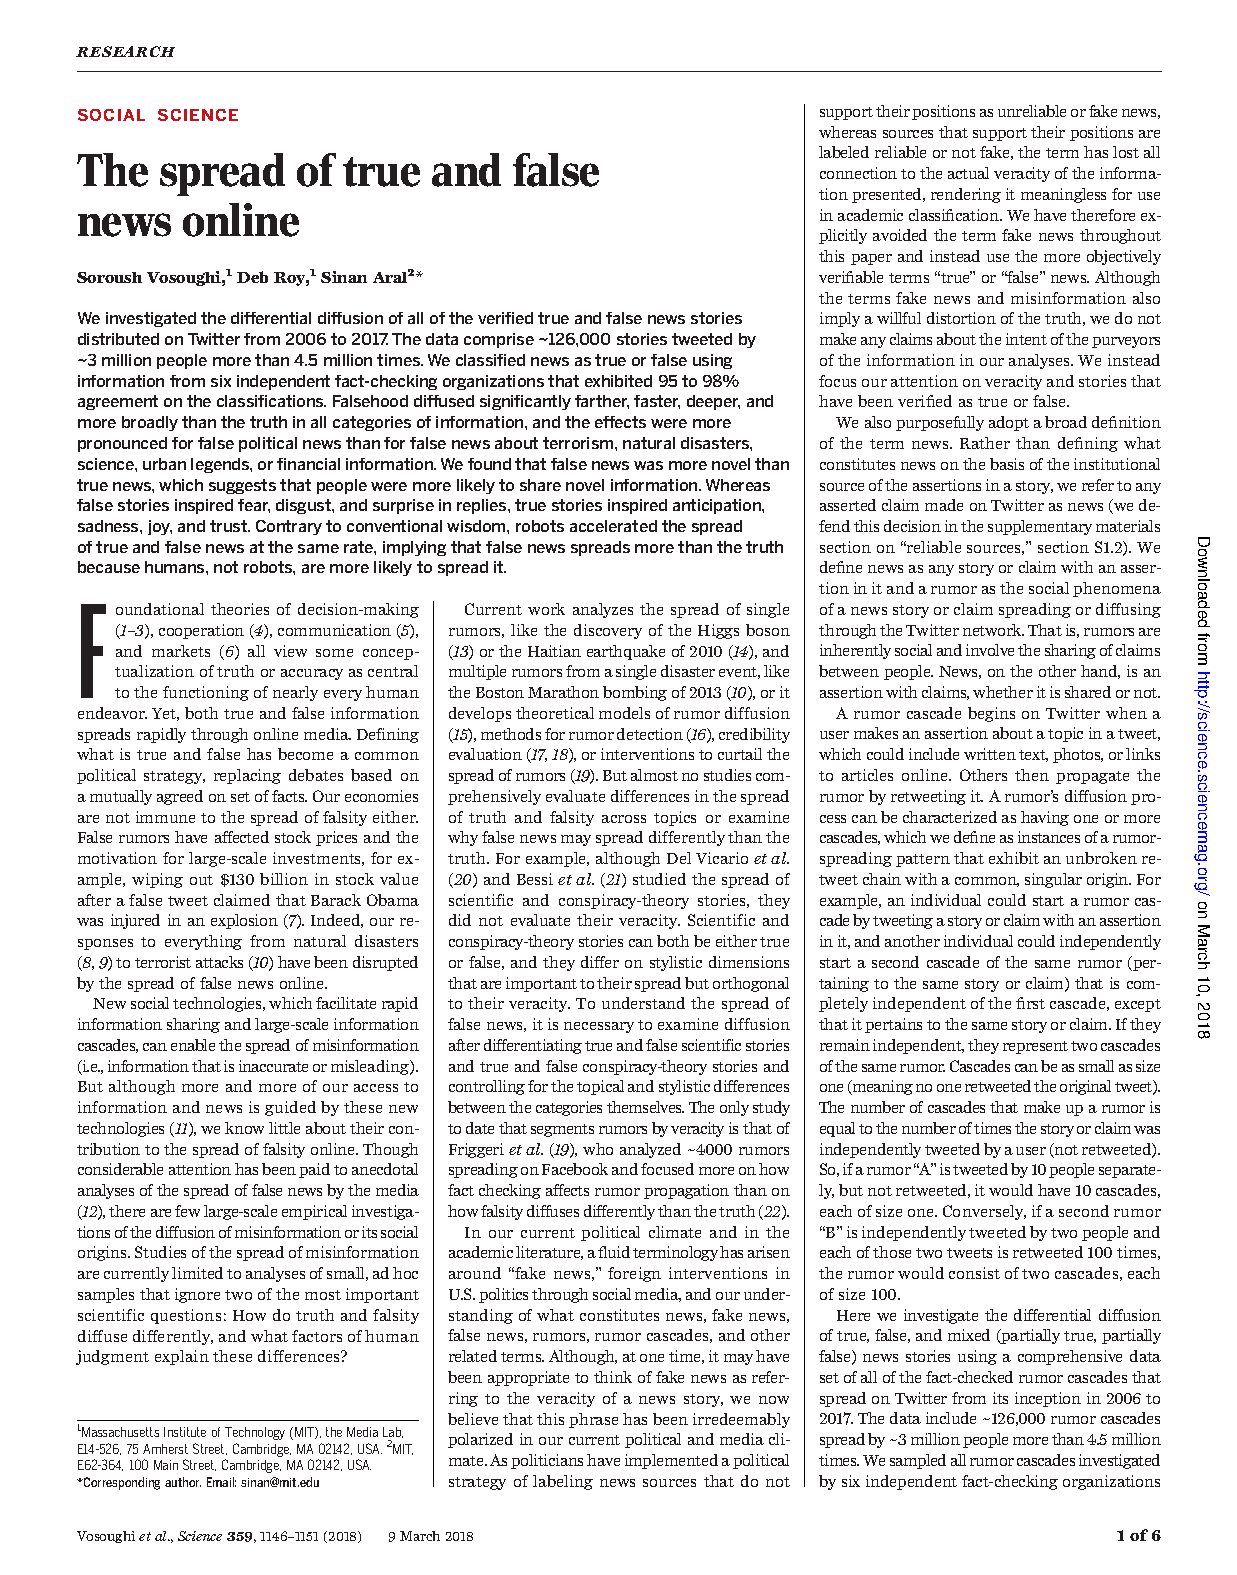
\includepdf[pages=1, scale=0.95, pagecommand=\heiti\sanhao{外\quad{}文\quad{}原\quad{}文}]{docs/translation.pdf}
\includepdf[pages=2-, scale=0.95, pagecommand={}]{docs/translation.pdf}
\end{center}

% 开题报告
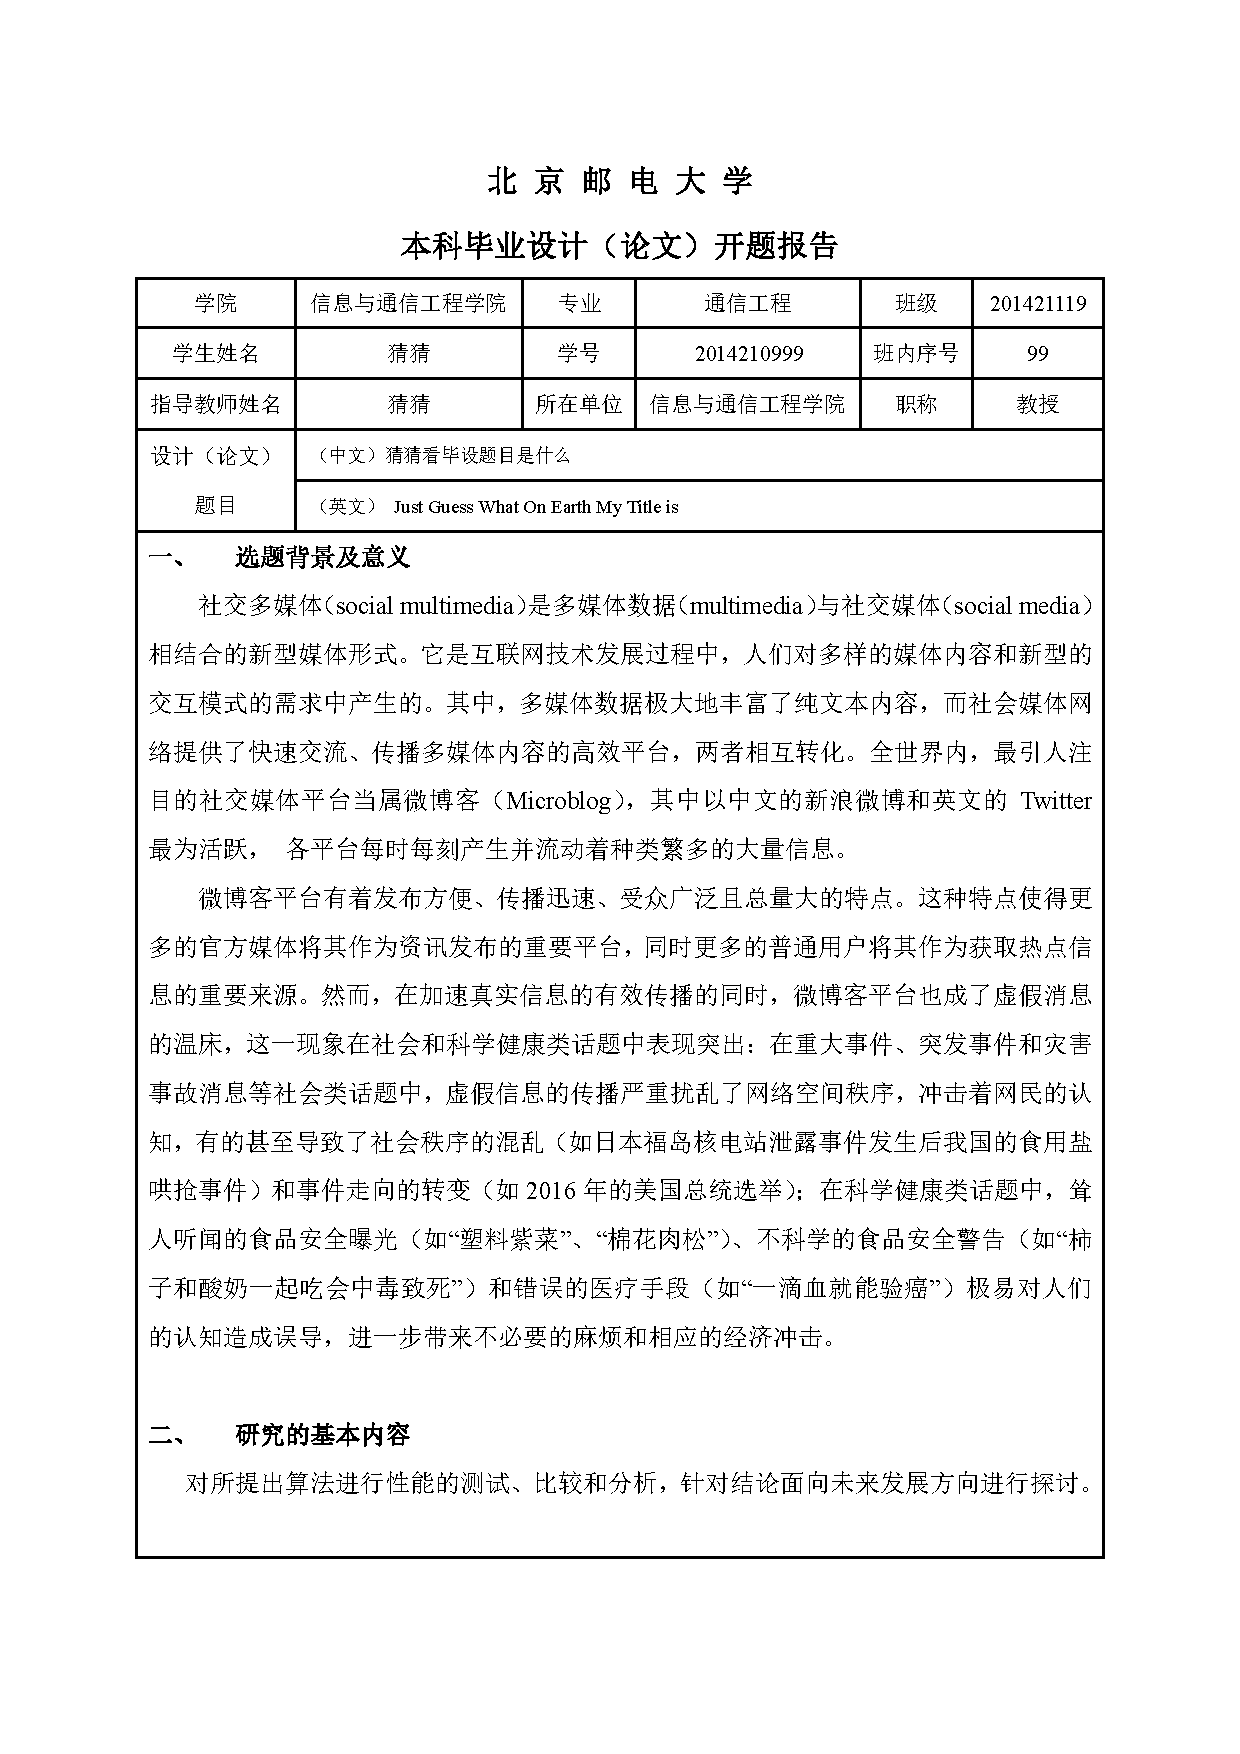
\includepdf[pages=-]{docs/openingReport.pdf} 


% 中期检查表
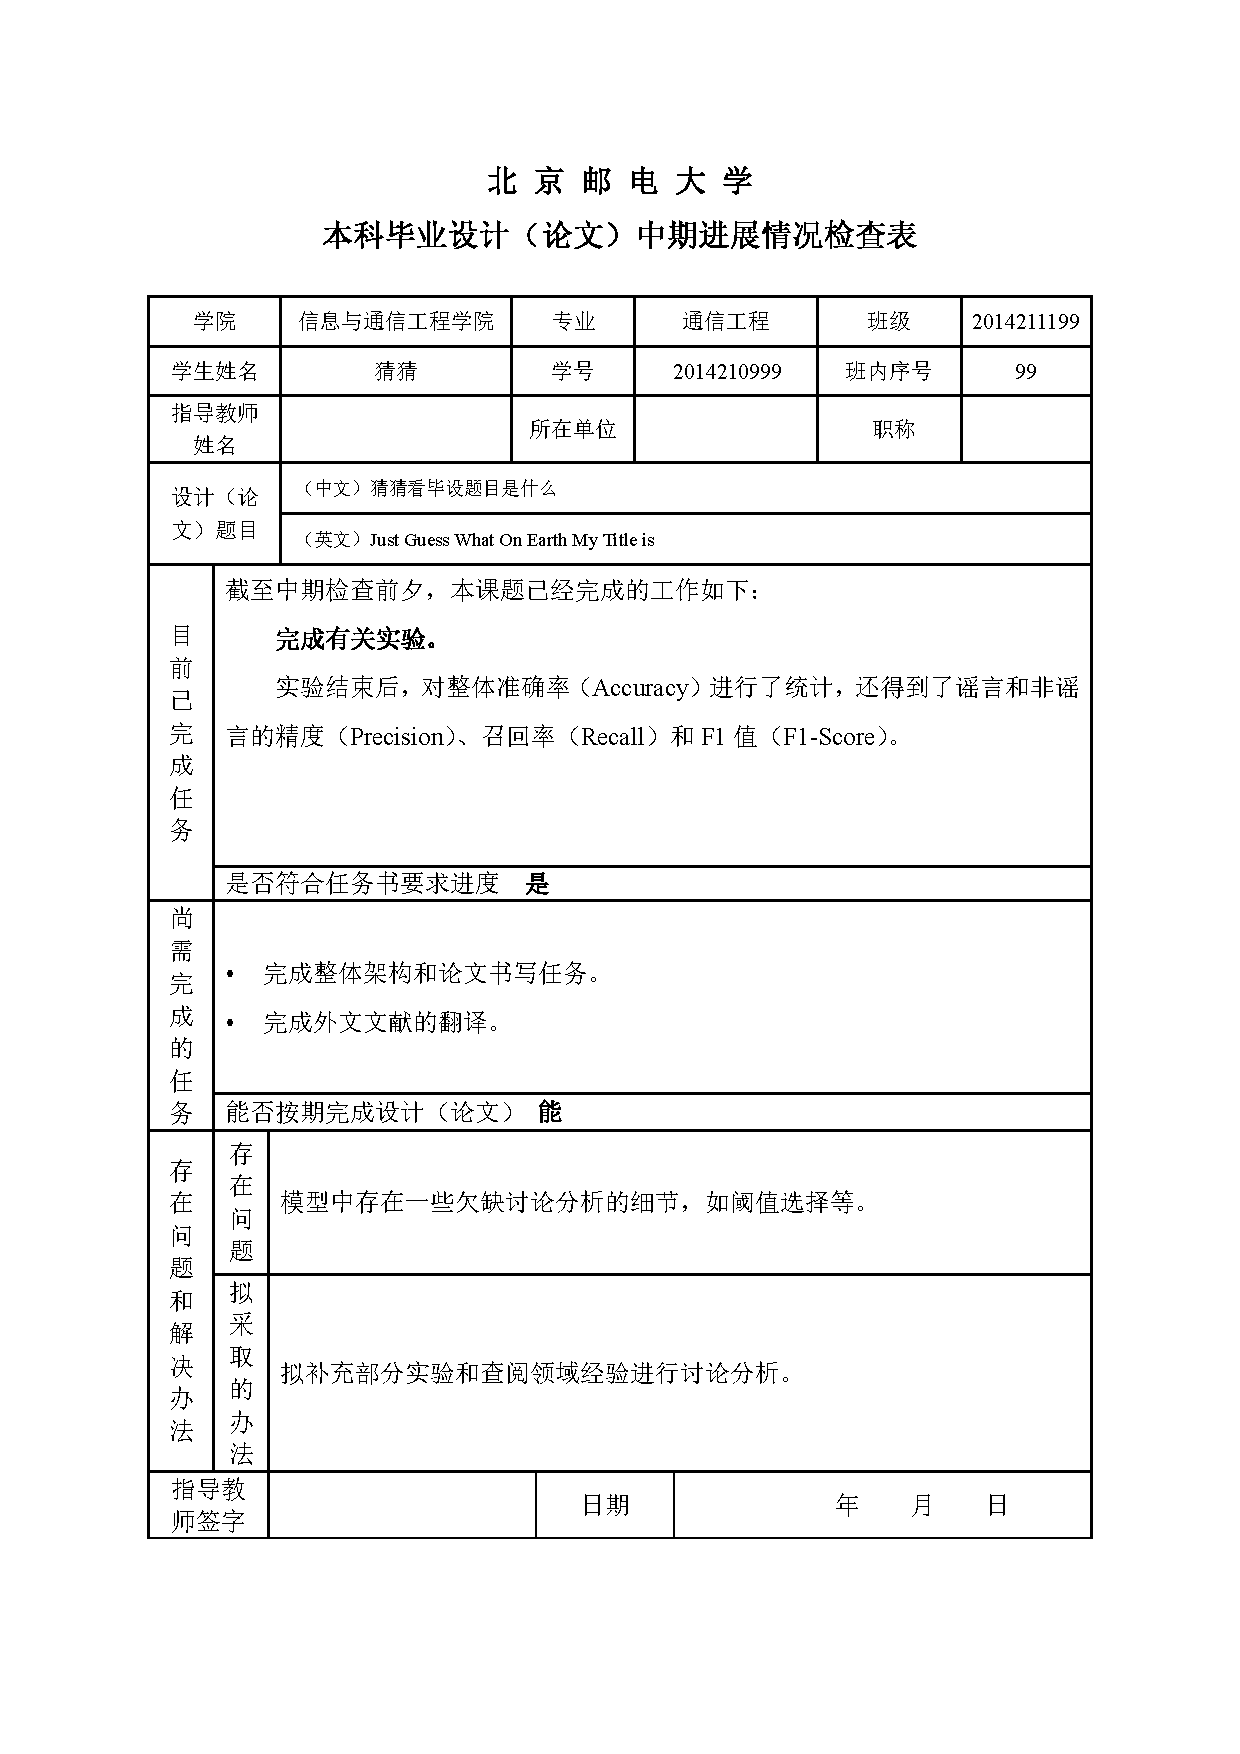
\includepdf[pages=-]{docs/interimReport.pdf} 


\end{document}